\section{Benchmark}

\subsection{lmapper VS kmapper}
We benchmarked lmapper against Kepler Mapper. To benchmark it a specific cover was implemented in \lstinline|lmapper.cover.KeplerCover| in order to implement the same method to build the cover. In both cases the filter used is a projection, since Kepler Mapper do not implement the Eccentricity filter. For this reason it is not possible to take advantage of the \lstinline|filterutils| package. As a clustering algorithm it was used a single linkage algorithm, where for lmapper the \lstinline|cutoff.FirstGap| class has been used to find the number of clusters, whereas for kmapper it was only possible to set a predetermined number of clusters, that has been chosen to be 2. Note that the performances of \lstinline|lmapper| are highly dependent on the parameter chosen to initialize \lstinline|cutoff.FirstGap|. Specifically, the smaller the parameter, the more clusters will be created and the slower will be the method \lstinline|complex.Complex.fit| affecting the overall performances of the package. For this benchmark this parameter has been set in order to obtain a graph the most similar to the one obtained by Kepler Mapper.

\textbf{Hardware used}:
Mac Book Pro late 2011 13", with a 32 nm "Sandy Bridge" 2.4 GHz Intel "Core i5" processor (2435M), 8 GB of 1333 MHz DDR3 SDRAM in two modules of 4GB each.

\begin{figure}[h]
	\caption{Synthetic dataset: performance comparison}
	\centering
	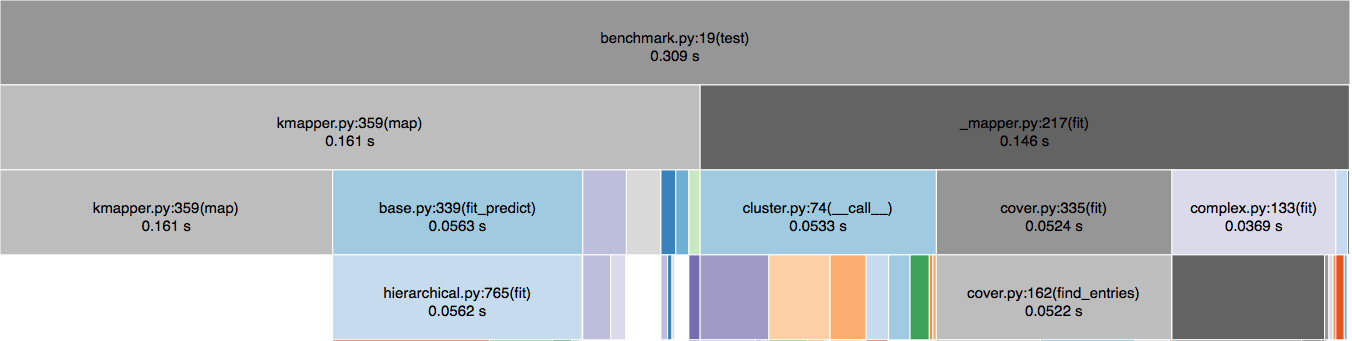
\includegraphics[width=0.9\textwidth]{images/benchmark/synthetic/benchmark}
\end{figure}
\begin{figure}[h!]
	\caption{Synthetic dataset: Left: graph obtained with Kepler Mapper. Right: graph obtained with lmapper}
	\centering
	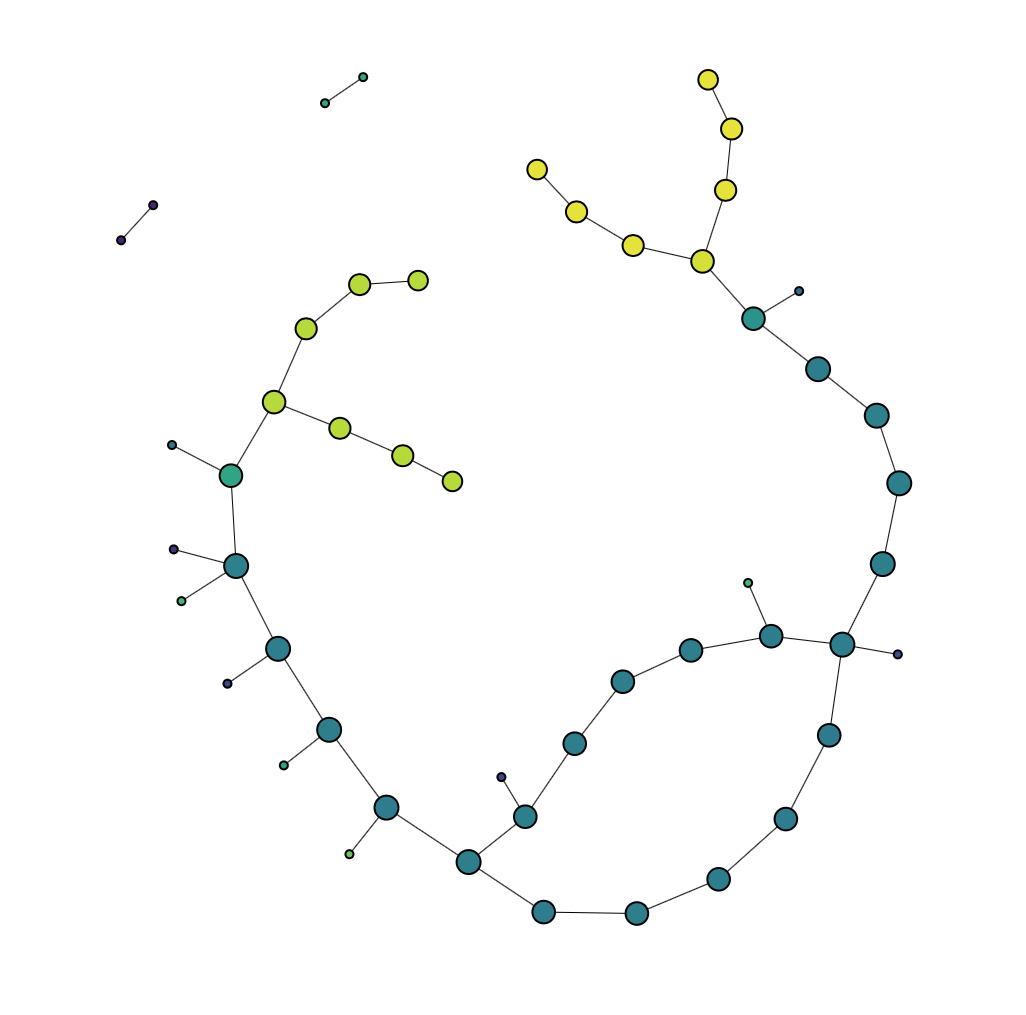
\includegraphics[width=0.4\textwidth]{images/benchmark/synthetic/benchmark_kmapper}
	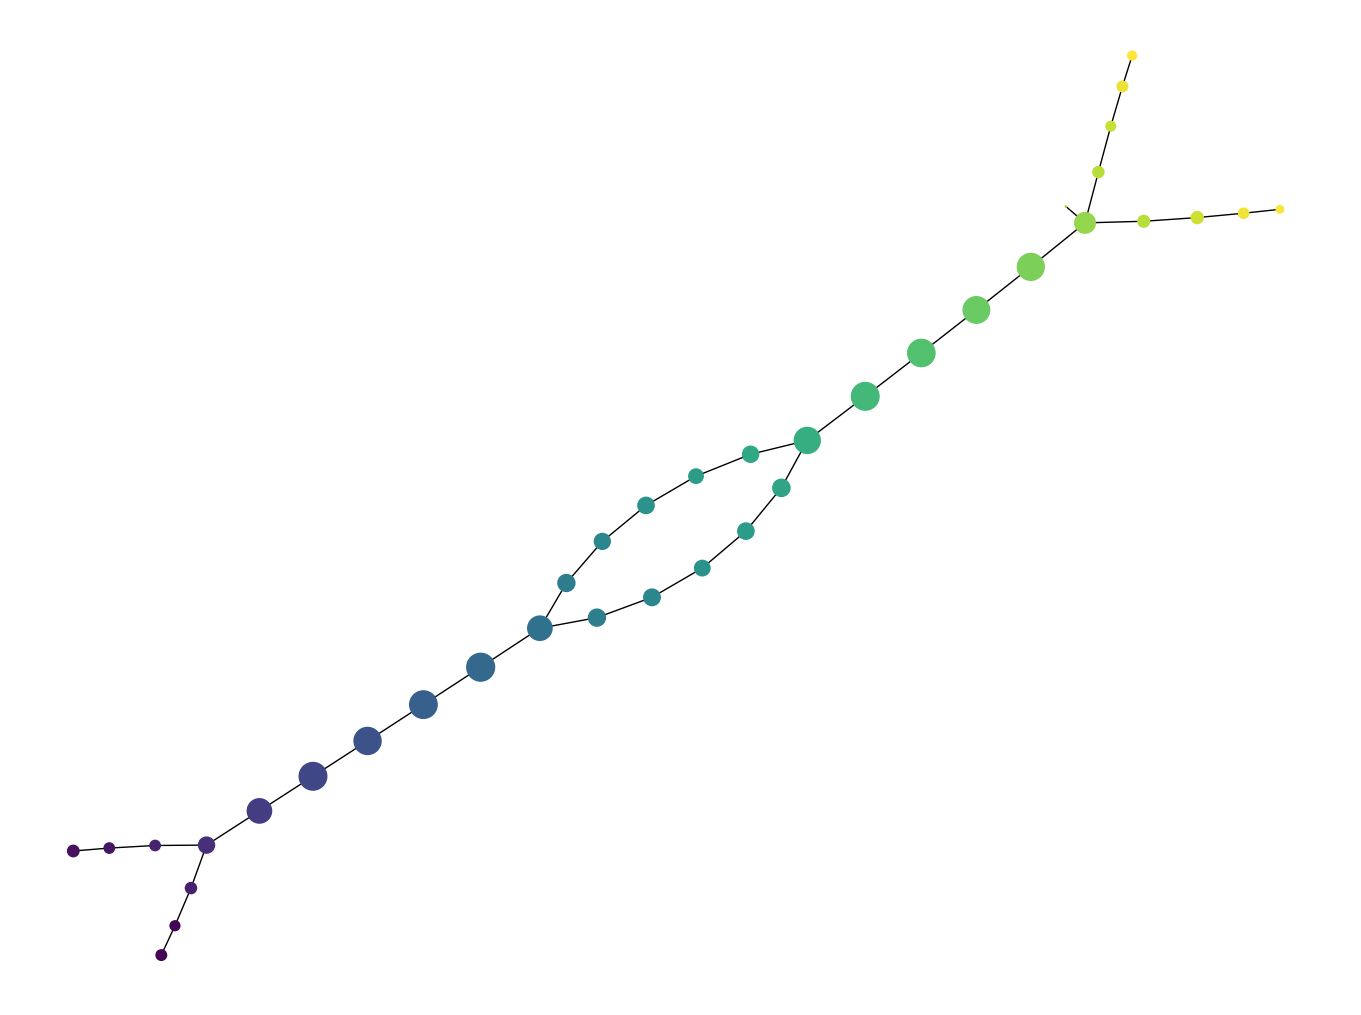
\includegraphics[width=0.4\textwidth]{images/benchmark/synthetic/benchmark_lmapper}
\end{figure}


On the synthetic dataset lmapper managed to get approximately a 10\% speedup compared to kmapper. The main topological features (the four branches and the ring at the center of the data point cloud) are correctly identified by both packages; furthermore we can see how the graph output of lmapper has much less noise than the graph obtained by kmapper. In the graph output of kmapper there are two small extra connected components, plus there are many little nodes connected to the biggest connected component. This was possible thanks to the class lmapper.cutoff.FirstGap that for each set of the cover calculates the number of clusters (nodes) to create from the dendrogram; in kmapper the number of clusters has to be fixed; in this case it was set to 2. This is what causes the creation of many little nodes (noise) in the kmapper output.

In conclusion, lmapper is faster and more robust to noise.

\begin{figure}[h]
	\caption{Wisconsin breast cancer dataset: performance comparison}
	\centering
	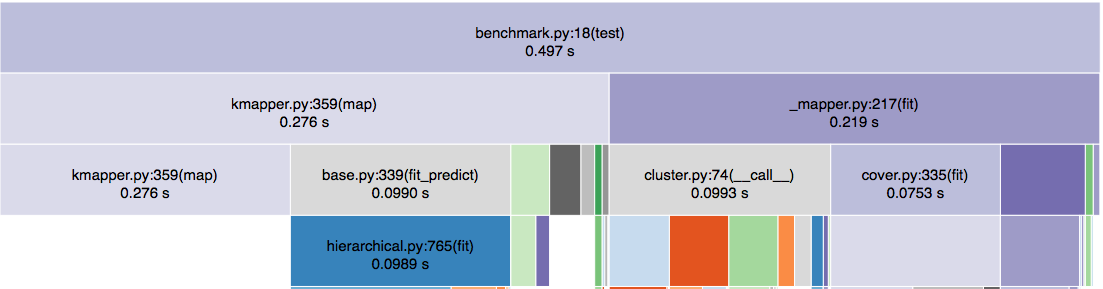
\includegraphics[width=0.9\textwidth]{images/benchmark/cat/benchmark}
\end{figure}
\begin{figure}[h!]
	\caption{Wisconsin breast cancer dataset. Left: graph obtained with Kepler Mapper. Right: graph obtained with lmapper}
	\centering
	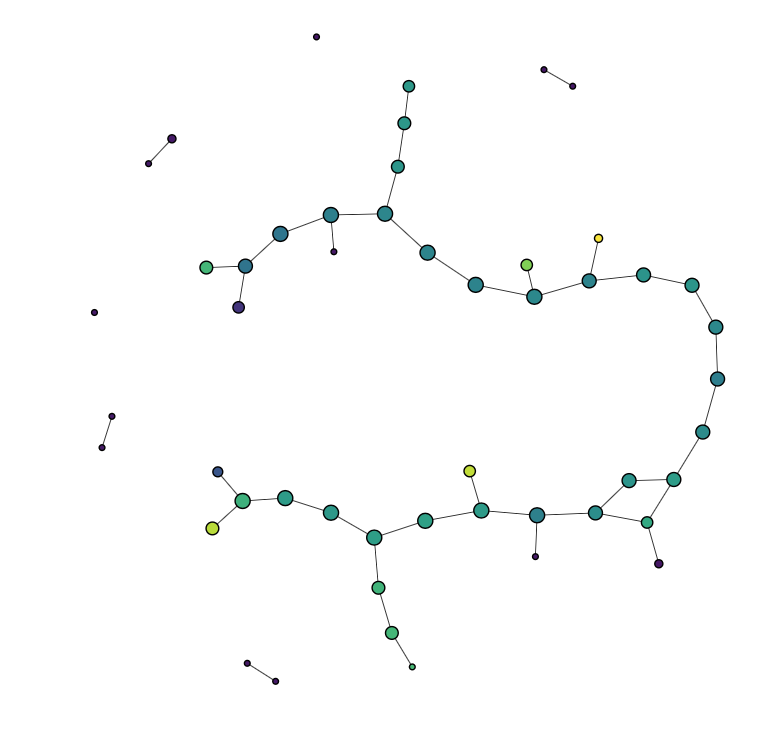
\includegraphics[width=0.4\textwidth]{images/benchmark/cat/benchmark_kmapper}	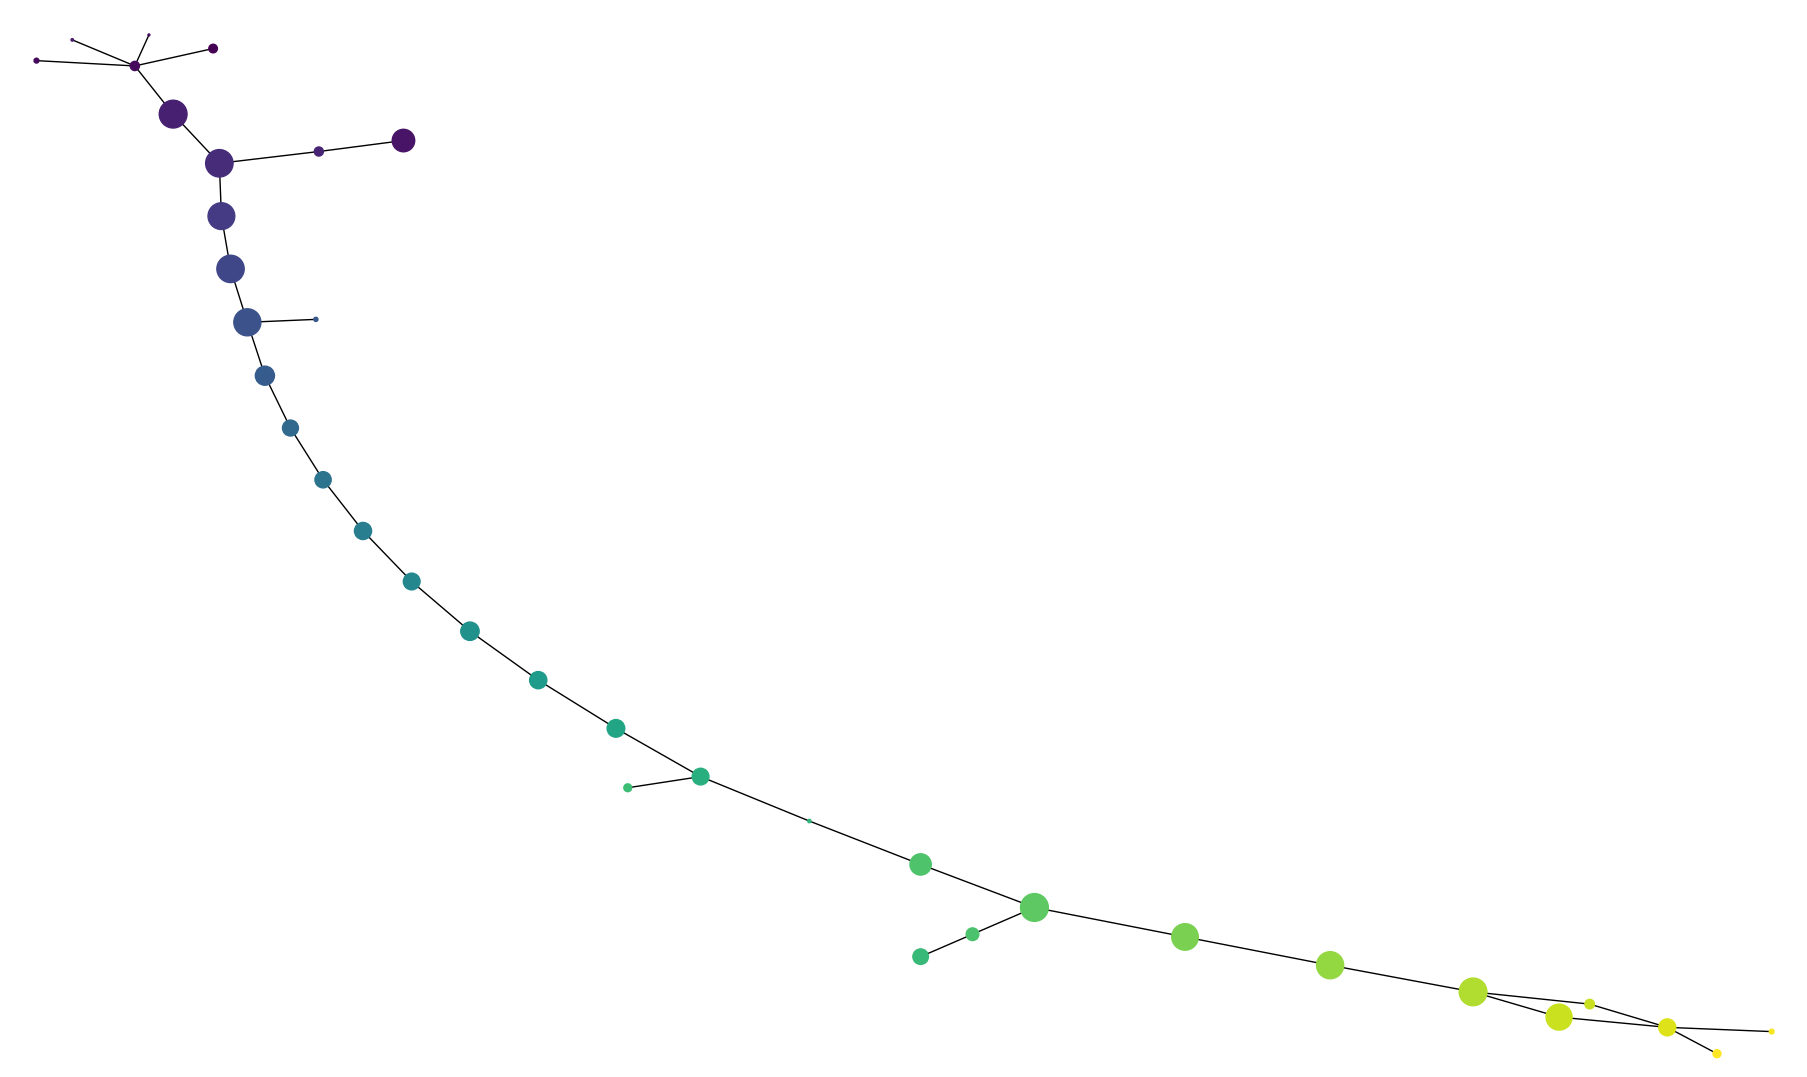
\includegraphics[width=0.4\textwidth]{images/benchmark/cat/benchmark_lmapper}
\end{figure}

On this second dataset lmapper is approximately 20\% faster than kmapper; again we see that lmapper's graph is again more robust to noise. There's only one connected component, and the main topological feature (the ring) is still captured.

\subsection{filterutils}
The filterutils package manage to get the following speedup:

\begin{center}
	
	\begin{tabular}{ cc } 
		
		Threads & Speedup \\ 
		\hline
		1& 1\\ 
		2 & 1.6 \\ 
	\end{tabular}\\
	\bigskip
	Accuracy
\end{center}

To see the results, execute the test\_filterutils.py file in the lmapper test folder. On our machine we were limited to only 1 and 2 threads, but it would be interesting to test the scalability of the package on machine with many cores.
\subsection{predmap}
With predmap we managed to obtain the same results of Francesco Palma's master thesis (see the test folder of the package)
Here a table confronting the results. The small differences in the synthetic datasets are due to the fact that the dataset is not exactly the same used in Palma's work, since it has been regenerated through a random process and thus it is slightly different. The difference in the Wisconsin dataset however means that there's some slight difference in the algorithms. 

\begin{center}
	
	\begin{tabular}{ ccc } 
	
		&Palma's results & predmap \\ 
		\hline
		Synthetic dataset & 71.01\% & 70.80\% \\ 
		Wisconsin breast cancer dataset & 79.10\% & 79.78\% \\ 
	\end{tabular}\\
\bigskip
	Accuracy
\end{center}

\paragraph{Conclusions}
To conclude, the pure Python implementation of lmapper obtained a speedup of 10\% and 20\% compared to Kepler Mapper on the synthetic dataset of Palma and the Cat dataset of \cite{pythonmapper}. filterutils shows good speedup in calculating the eccentricity filter. Thanks to the implementation of the cutoff in the cutoff.py module the output is more robust to noise. predmap was capable of reproducing very closely the results of Francesco Palma's master thesis.
